\documentclass[10pt,a4paper]{article}

% Packages
\usepackage[utf8]{inputenc}
\usepackage{amsmath}
\usepackage{amsfonts}
\usepackage{amssymb}
\usepackage{graphicx}
\usepackage{hyperref}
\usepackage{cite}
\usepackage{algorithm}
\usepackage{algorithmic}
\usepackage{listings}
\usepackage{xcolor}
\usepackage[margin=0.75in]{geometry}
\usepackage{multicol}
\usepackage{caption}

% Prevent hyphenation of specific words
\hyphenation{tracking}

% Document information
\title{Edge-Oriented Visual Object Tracking Based on Confidence-Aware CSRT with Kalman Filtering and Lightweight Deep Scale Refinement}

\date{}

\begin{document}

\maketitle

{\small
\begin{abstract}
Visual object tracking remains challenging under appearance variation, occlusion, scale change, fast motion, and background clutter, especially when real-time or embedded deployment is required. The Channel and Spatial Reliability Tracker (CSRT) is a strong classical correlation-filter tracker with efficient online performance, making it a suitable lightweight baseline for practical tracking; however, its response-driven localization and fixed update strategy may lead to drift when the response map becomes ambiguous or unreliable. This paper proposes CA-CSRT, a Confidence-Aware CSRT framework that enhances the standard CSRT pipeline by integrating Kalman-based motion prediction, APCE-based response reliability estimation, confidence-guided measurement fusion, lightweight local scale refinement, and confidence-controlled model update. The Kalman filter first provides a motion-guided target center, and the local refinement module then predicts log-scale corrections for bounding-box width and height without performing full-frame detection. On the laptop-based OTB100 evaluation, CA-CSRT improves average Success AUC over pure CSRT from 53.12 to 54.00 and achieves higher AUC on 57/100 sequences. On the server-based LaSOT evaluation, CA-CSRT improves average Success AUC from 16.73 to 22.88 and achieves higher AUC on 27/40 sequences. Runtime evaluation reports 62.2 FPS on OTB100 using the laptop platform, 75.03 FPS on the LaSOT evaluation using the server platform, and 22.76 FPS on Jetson Nano B01, indicating that CA-CSRT improves the robustness-efficiency trade-off while remaining practical for lightweight embedded visual tracking.
\end{abstract}

\noindent\textbf{Keywords:} Visual Object Tracking, CSRT, Correlation Filter, Kalman Filtering, Confidence-Aware Tracking, Deep Feature Refinement, Embedded Vision.
}

\vspace{0.3cm}

\begin{multicols}{2}

\section{Introduction}

Visual object tracking estimates the position and scale of a target throughout a video sequence from its initial state. Robust tracking remains challenging under fast motion, partial occlusion, scale variation, illumination change, background clutter, and target deformation, especially when real-time or embedded deployment requires a practical balance between accuracy, robustness, and efficiency.

Correlation filter-based trackers are widely used because they offer efficient online localization. The Channel and Spatial Reliability Tracker (CSRT) improves this family by using spatial reliability masks and channel-wise weighting, making it a strong classical baseline for practical tracking. However, CSRT remains mainly response-driven: the target location is inferred from the correlation response peak, and the appearance model is updated according to a predefined online strategy.

When the response map becomes ambiguous because of occlusion, abrupt motion, appearance deformation, or background distractors, the dominant peak may no longer correspond reliably to the target. In such cases, directly using the visual response can introduce localization error, and updating the model with an unreliable observation can contaminate the appearance representation and increase the risk of drift.

This paper proposes CA-CSRT, a Confidence-Aware CSRT framework designed to improve the robustness-efficiency trade-off of a CSRT-family tracker. CA-CSRT combines Kalman-based motion prediction, response-confidence estimation, confidence-guided measurement fusion, lightweight local scale refinement, and confidence-controlled model update. The design supports practical deployment by adding reliability-aware control while preserving an efficient online tracking structure suitable for lightweight platforms such as Jetson Nano.

The main contributions are summarized as follows:
\vspace{-0.4em}
\begin{itemize}
    \setlength{\itemsep}{0.1em}
    \setlength{\parskip}{0pt}
    \setlength{\parsep}{0pt}
    \setlength{\topsep}{0.1em}
    \item We propose CA-CSRT, a confidence-aware CSRT-family tracker that integrates correlation localization with Kalman-based motion prediction.
    \item We use response confidence to guide measurement fusion and conservative model update under unreliable observations.
    \item We incorporate lightweight local scale refinement to improve bounding-box stability without full-frame detection at every frame.
    \item We evaluate CA-CSRT on OTB100, an evaluated LaSOT subset, FPS--AUC trade-off, and Jetson Nano deployment.
\end{itemize}

\section{Related Works}

\subsection{Correlation Filters and Motion Modeling}

Correlation filter-based trackers provide a favorable balance between localization accuracy and computational efficiency. MOSSE [1] introduced adaptive correlation filtering for fast visual tracking, and KCF [2] further improved efficiency by exploiting circulant structure and Fourier-domain computation. These methods demonstrate why correlation filters remain attractive when online adaptation and high frame rates are required.

CSRT [3] improves correlation-filter localization with spatial reliability masks and channel reliability weights, which help suppress background interference and emphasize more discriminative feature channels. However, CSRT still estimates the target mainly from the response peak and updates the appearance model using a predefined strategy. Flat, noisy, or multi-modal responses caused by occlusion, fast motion, appearance deformation, or background distractors can therefore produce inaccurate measurements and model drift. Kalman filtering [5] provides a lightweight motion prior for temporal consistency, but fixed fusion between motion prediction and visual measurement is not always suitable. CA-CSRT addresses this issue by using response confidence to balance CSRT localization and Kalman prediction, so unreliable visual measurements are treated more conservatively.

\subsection{Deep Feature-Based Tracking}

Deep features and modern Siamese or transformer-based trackers can improve visual representation, especially under large appearance variation and clutter. However, many such trackers introduce computational cost and memory demand that can be difficult to deploy on resource-constrained hardware. Hybrid designs therefore integrate lightweight deep components into efficient classical trackers instead of replacing the full pipeline.

For correlation-filter trackers, auxiliary deep refinement can support appearance representation, scale estimation, or bounding-box adjustment. Scale variation is important because inaccurate target size directly affects overlap-based success and can degrade the following model update. DSST [4] addresses scale adaptation with a dedicated estimator, while CA-CSRT follows a hybrid idea by using lightweight local refinement within a motion-guided region. The refinement is restricted to the neighborhood of the fused target center rather than running full-frame detection, which helps preserve the efficiency of the CSRT-family pipeline.

\section{Proposed Method}

\subsection{Overview of the Proposed CA-CSRT Framework}

Given an initial bounding box $B_0=(x_0,y_0,w_0,h_0)$, visual tracking estimates $B_k=(x_k,y_k,w_k,h_k)$ for each frame $k$. CA-CSRT formulates this process as a motion-guided and confidence-controlled closed loop that combines correlation localization, motion prediction, response reliability estimation, scale refinement, and model update.

For each frame, a Kalman filter predicts the target state and defines a motion-guided search region. CSRT-based correlation localization is then applied inside this region to obtain a visual measurement from the response map. The response quality is evaluated using peak-based confidence, especially APCE, and the resulting confidence controls the fusion between the CSRT measurement and the Kalman prediction.

After APCE-guided Kalman fusion, the fused target center is used to define a local refinement crop. The lightweight deep refinement module is then applied only to this local region to adjust the target scale and aspect ratio. Thus, the CNN refinement component is not a separate localization branch; it operates after the center has been estimated and refines only the bounding-box size. The same confidence score also affects the model update: reliable observations can update the appearance model, while low-confidence observations are treated conservatively to reduce model contamination. The overall architecture is illustrated in Figure~\ref{fig:ca_csrt_pipeline}.

\end{multicols}
\vspace{-0.35cm}
\begin{center}
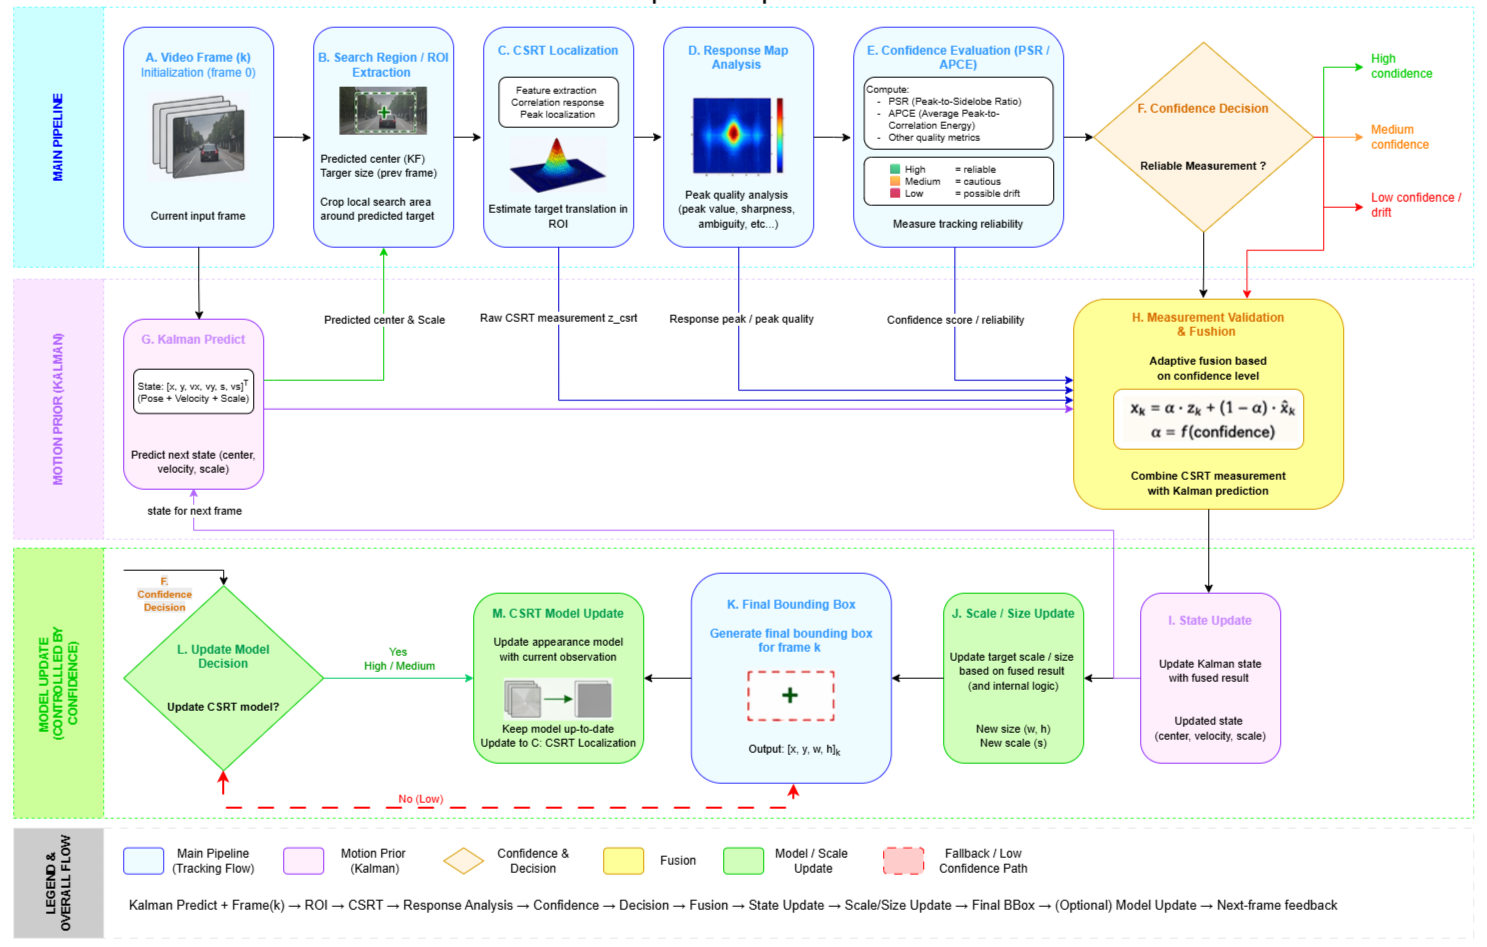
\includegraphics[width=0.65\textwidth]{Bao_CSRTUpdate_OnlyDraio1.drawio.png}
\captionof{figure}{Overall architecture of the proposed CA-CSRT pipeline.}
\label{fig:ca_csrt_pipeline}
\end{center}
\vspace{-0.35cm}
\begin{multicols}{2}

\subsection{Correlation-Based Localization Using CSRT}

Within the motion-guided search region, CA-CSRT uses a CSRT-family localization module to obtain a visual measurement rather than the final target state. Let $x_k \in \mathbb{R}^{H \times W \times C}$ denote the multi-channel feature representation at frame $k$. The CSRT localization process can be abstracted as learning channel-wise filters $\{f_c\}_{c=1}^{C}$ with a spatial reliability constraint:

\begin{equation}
\min_{\{f_c\}} \sum_{c=1}^{C}
\left\| m \odot (x_{k,c} * f_c - y) \right\|^2
+ \lambda \left\| f_c \right\|^2 ,
\end{equation}
where $m$ denotes the spatial reliability mask, $y$ is the desired Gaussian-shaped response, $\lambda$ is the regularization parameter, and $*$ denotes correlation.

The response map is computed as a weighted combination of channel responses:

\begin{equation}
R_k = \sum_{c=1}^{C} w_c \cdot (x_{k,c} * f_c),
\end{equation}
where $w_c$ is the reliability weight of the $c$-th channel. Its peak gives the raw CSRT center estimate:

\begin{equation}
c_k^{\mathrm{CSRT}} = \arg\max_{p} R_k(p),
\end{equation}
which is represented as the measurement vector
$z_k^{\mathrm{CSRT}} = [x_k^{\mathrm{CSRT}}, y_k^{\mathrm{CSRT}}]^{\top}$.

Because $z_k^{\mathrm{CSRT}}$ can be unreliable under fast motion, occlusion, deformation, or background distractors, CA-CSRT further analyzes $R_k$ before Kalman fusion and model update.

\subsection{APCE-Based Measurement Reliability Estimation}

The CSRT response map $R_k$ also indicates measurement reliability. CA-CSRT estimates this reliability using APCE, which measures response sharpness and contrast:

\begin{equation}
\mathrm{APCE}_k =
\frac{\left(R_k^{\max}-R_k^{\min}\right)^2}
{\frac{1}{|R_k|}\sum_i \left(R_k(i)-R_k^{\min}\right)^2 + \epsilon},
\end{equation}
where $R_k^{\max}$ and $R_k^{\min}$ are the maximum and minimum response values, $|R_k|$ is the number of response locations, and $\epsilon$ prevents numerical instability. High APCE usually indicates a sharp dominant peak and a more reliable visual measurement. Low APCE may correspond to a flat, noisy, or multi-modal response caused by occlusion, fast motion, appearance deformation, or background distractors. APCE is used here as an internal confidence cue for online tracking control, not as an external benchmark metric. The score is converted into a normalized confidence coefficient:

\begin{equation}
\alpha_k = \sigma\left(\beta(\mathrm{APCE}_k-\tau)\right),
\end{equation}
where $\sigma(\cdot)$ is the sigmoid function, $\tau$ is the confidence threshold, and $\beta$ controls transition sharpness. The coefficient $\alpha_k \in [0,1]$ controls measurement fusion and conservative model update.

\subsection{Kalman Filter with APCE-Guided Measurement Fusion}

CA-CSRT uses a constant-velocity Kalman filter as a lightweight motion prior. The state is:

\begin{equation}
\mathbf{s}_k = [x_k, y_k, \dot{x}_k, \dot{y}_k]^{\top},
\end{equation}
where $(x_k,y_k)$ is the target center and $(\dot{x}_k,\dot{y}_k)$ is velocity. Prediction is performed by:

\begin{equation}
\hat{\mathbf{s}}_{k|k-1} = \mathbf{F}\hat{\mathbf{s}}_{k-1|k-1},
\end{equation}
\begin{equation}
\mathbf{P}_{k|k-1} = \mathbf{F}\mathbf{P}_{k-1}\mathbf{F}^{\top} + \mathbf{Q},
\end{equation}
where $\mathbf{F}$ is the state transition matrix, $\mathbf{P}_{k|k-1}$ is the predicted covariance, and $\mathbf{Q}$ is process noise. The predicted center defines the search region for CSRT localization. The raw CSRT center is treated as the visual measurement:

\begin{equation}
\mathbf{z}_k^{\mathrm{CSRT}} =
[x_k^{\mathrm{CSRT}}, y_k^{\mathrm{CSRT}}]^{\top}.
\end{equation}
Instead of a fixed measurement noise covariance, CA-CSRT adapts it using $\alpha_k$:

\begin{equation}
\mathbf{\Sigma}^{z}_k =
\frac{1}{\alpha_k+\epsilon}\mathbf{\Sigma}^{z}_0,
\end{equation}
where $\mathbf{\Sigma}^{z}_0$ is nominal measurement noise. High $\alpha_k$ reduces covariance and trusts the visual measurement more, while low $\alpha_k$ increases covariance and relies more on the motion prior. The Kalman gain is:

\begin{equation}
\mathbf{K}_k =
\mathbf{P}_{k|k-1}\mathbf{H}^{\top}
(\mathbf{H}\mathbf{P}_{k|k-1}\mathbf{H}^{\top}
+ \mathbf{\Sigma}^{z}_k)^{-1},
\end{equation}
where $\mathbf{H}$ maps the state to the measured center. The fused state is:

\begin{equation}
\hat{\mathbf{s}}_k =
\hat{\mathbf{s}}_{k|k-1}
+ \mathbf{K}_k
(\mathbf{z}_k^{\mathrm{CSRT}} - \mathbf{H}\hat{\mathbf{s}}_{k|k-1}).
\end{equation}
This update lets reliable responses correct the prediction more strongly, while ambiguous responses produce more conservative state updates.

\subsection{Deep Feature--Based Scale Refinement}

After APCE-guided Kalman fusion provides the target center, CA-CSRT uses this fused center to crop a local refinement region. The lightweight deep refinement module operates only on this local crop to adjust target scale and aspect ratio. It does not perform full-frame localization and does not estimate the target center independently; instead, it refines the bounding-box size after the center has already been determined by the CSRT--Kalman fusion stage. Let $\Omega_k$ denote the local crop around the fused center. The module estimates relative size change using log-scale ratios:
\begin{equation}
y_w = \log \frac{w_k}{w_{k-1}}, \qquad
y_h = \log \frac{h_k}{h_{k-1}} .
\end{equation}
The CNN therefore learns a relative log-scale correction for the bounding-box width and height, rather than directly predicting a new target location.
With predicted log-scale ratios $(\mu_w,\mu_h)$, the refined size is:
\begin{equation}
w_k^{\mathrm{ref}} = w_{k-1}\exp(\mu_w), \qquad
h_k^{\mathrm{ref}} = h_{k-1}\exp(\mu_h).
\end{equation}
The final size is smoothed to avoid abrupt changes:
\begin{equation}
\begin{aligned}
w_k &= (1-\eta_k)w_{k-1} + \eta_k w_k^{\mathrm{ref}},\\
h_k &= (1-\eta_k)h_{k-1} + \eta_k h_k^{\mathrm{ref}},
\end{aligned}
\end{equation}
where $\eta_k \in [0,1]$ controls the scale update rate. This module is used only as a local inference-time refinement and is decoupled from CSRT filter learning, avoiding online back-propagation or full-frame detector updates. In this design, deep refinement complements the CSRT response-based localization by improving bounding-box stability rather than replacing the correlation-filter localization core.

\subsection{Closed-Loop Model Update}

After APCE-guided fusion and scale refinement, CA-CSRT obtains:
\begin{equation}
B_k = (x_k,y_k,w_k,h_k).
\end{equation}
The final box is fed back for the next frame and for CSRT appearance-model update. When $\alpha_k$ is high, the observation can be used for normal update; when $\alpha_k$ is low, CA-CSRT applies a conservative strategy such as reducing or skipping the update. This confidence-controlled loop links localization, reliability estimation, motion fusion, scale refinement, and model update, reducing the risk of drift while preserving the lightweight online structure of CSRT-family tracking.

\section{Experimental Results}

\subsection{Experimental Setup}

CA-CSRT is evaluated using the One-Pass Evaluation (OPE) protocol. OTB100~[7] is used as the primary short-term benchmark, while an evaluated LaSOT~[6] subset of 40 sequences is used for longer and more challenging videos; these LaSOT results are therefore subset results. Metrics include success AUC, Precision@20, FPS, and the FPS--AUC trade-off. Success AUC summarizes overlap-based tracking accuracy over different intersection-over-union thresholds, while Precision@20 measures the percentage of frames whose center error is below 20 pixels. FPS is used as a runtime indicator, and the FPS--AUC trade-off is emphasized because embedded tracking requires both acceptable robustness and deployable speed.

Laptop experiments were conducted on an ASUS Zenbook UX3402VA with a 13th Gen Intel Core i7-1360P processor and 16 GB RAM. Embedded deployment is evaluated on an NVIDIA Jetson Nano B01 platform.

\subsection{Overall FPS--AUC Trade-off on OTB100 and LaSOT}

CA-CSRT aims to improve the robustness-efficiency trade-off of a CSRT-family tracker. Figure~\ref{fig:fps_auc_cross_dataset} summarizes the relationship between tracking speed and success AUC on OTB100 and the evaluated LaSOT subset.

\end{multicols}
\vspace{-0.35cm}
\begin{center}
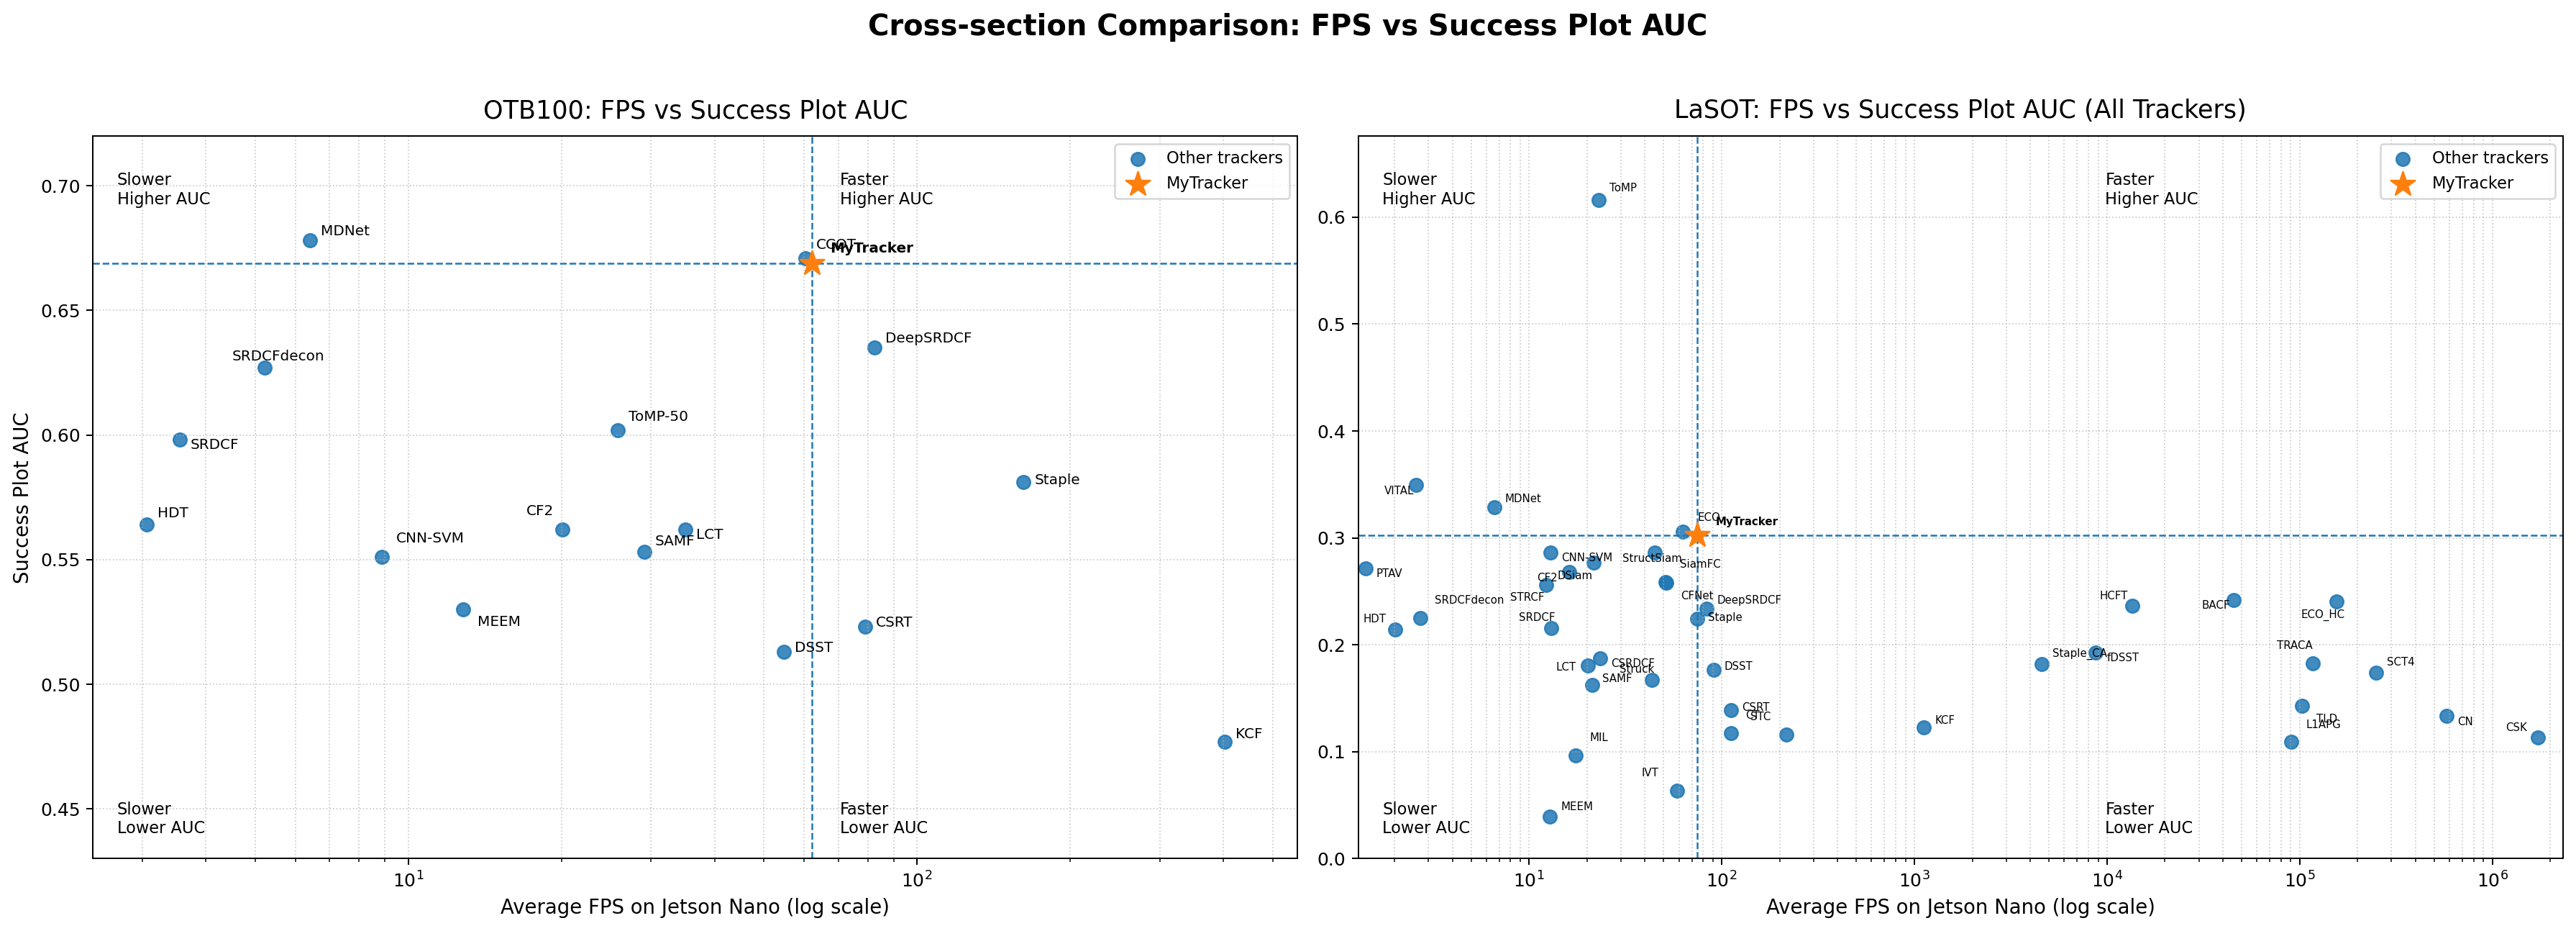
\includegraphics[width=0.72\textwidth]{otb100_lasot_fps_success_auc_cross_section_full_en.png}
\captionof{figure}{FPS--AUC comparison on OTB100 and the evaluated LaSOT subset.}
\label{fig:fps_auc_cross_dataset}
\end{center}
\vspace{-0.35cm}
\begin{multicols}{2}

The FPS--AUC comparison indicates that CA-CSRT operates in a practical runtime region while maintaining competitive success performance. Accuracy alone is insufficient for embedded tracking, where a high-accuracy but slow model may be less useful than a tracker that maintains acceptable robustness at deployable speed. This is consistent with the CA-CSRT design: Kalman prediction constrains the search region, APCE-based confidence reduces unreliable updates, and local refinement improves scale stability without full-frame detection.

Edge-oriented tracking literature also emphasizes the accuracy--speed trade-off. For example, Zhai et al. [8] report that STARK-S50 reaches 5.56 FPS on Jetson TX2, LightTrack 18 FPS, and MobileTrack more than 33 FPS, motivating embedded FPS and FPS--AUC analysis; these values are not directly compared with our Jetson Nano results because the hardware and implementations differ.

\subsection{Comparison with Pure CSRT}

CA-CSRT is compared with a pure CSRT baseline on OTB100 and the evaluated LaSOT subset. Table~\ref{tab:csrt_comparison_summary} summarizes the per-sequence AUC comparison.

\begin{center}
\scriptsize
\captionof{table}{AUC comparison between CA-CSRT and pure CSRT. AUC values are reported in percentage points.}
\label{tab:csrt_comparison_summary}
\resizebox{\columnwidth}{!}{%
\begin{tabular}{lccccc}
\hline
Dataset & N & CA/CSRT wins & CA AUC & CSRT AUC & $\Delta$AUC \\
\hline
OTB100 & 100 & 57/43 & 54.00 & 53.12 & +0.89 \\
LaSOT subset & 40 & 27/13 & 22.88 & 16.73 & +6.15 \\
\hline
\end{tabular}
}
\end{center}

On OTB100, CA-CSRT obtains a slightly higher mean AUC than pure CSRT, with 57 out of 100 sequences showing higher AUC. The mean gain is modest, which is consistent with the short-term nature of many OTB100 videos where a well-tuned pure CSRT baseline can already maintain reliable localization.

On the evaluated LaSOT subset, CA-CSRT obtains a larger mean AUC gain and wins on 27 out of 40 sequences. This suggests that confidence-aware fusion and update control are more beneficial in longer or more challenging sequences, where occlusion, target deformation, and accumulated update errors can have greater impact.

Pure CSRT still performs better on some sequences, so CA-CSRT should be interpreted as a robustness-oriented enhancement rather than a replacement that is better in every case. The comparison indicates improved average behavior under the evaluated settings, not universal sequence-wise superiority.

\subsection{Representative Challenge Sequence Analysis}

While Table~\ref{tab:csrt_comparison_summary} summarizes the average AUC comparison, representative challenge sequences provide a more detailed view of tracker behavior under different conditions. In the generated plots, the label ``MyTracker'' denotes the implemented CA-CSRT variant evaluated in this paper. The following visualizations are intended to support a balanced interpretation of CA-CSRT by illustrating both favorable and failure cases.

\vspace{-0.10cm}
\begin{center}
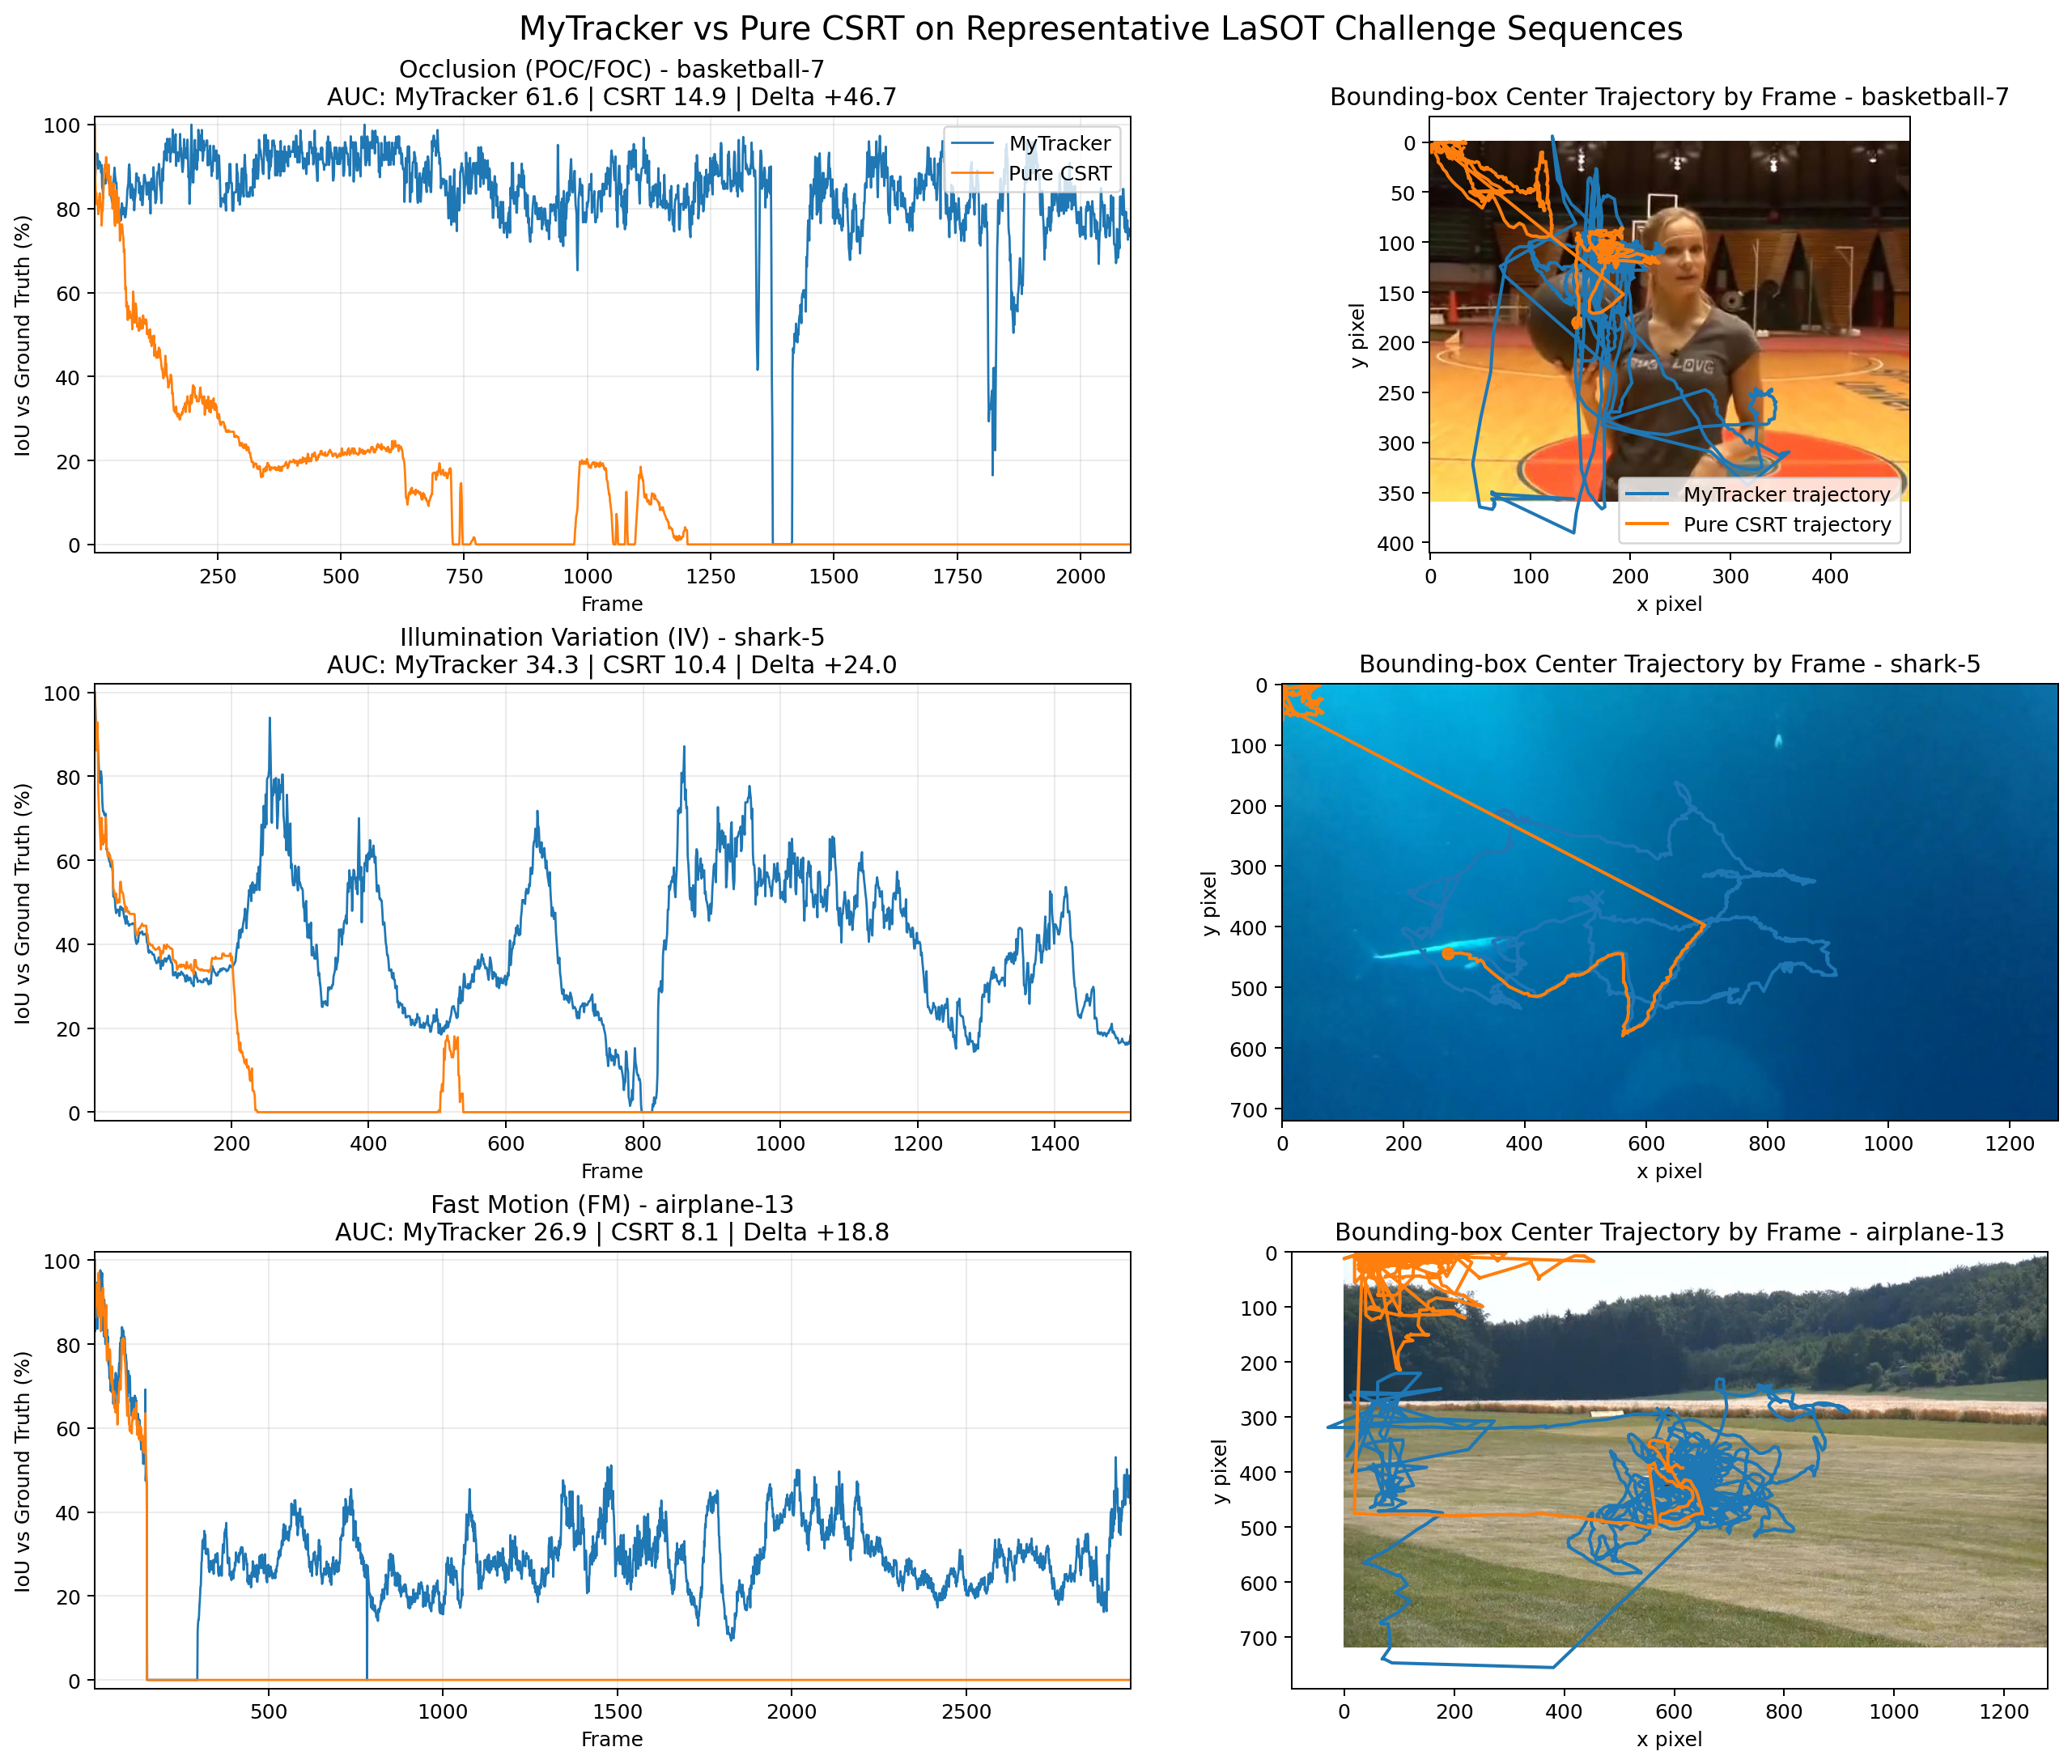
\includegraphics[width=0.94\columnwidth]{lasot_challenge_representative_mytracker_vs_csrt.png}
\captionof{figure}{Representative LaSOT challenge sequences comparing CA-CSRT and pure CSRT. The left panels show IoU over time, while the right panels show bounding-box center trajectories.}
\label{fig:lasot_representative_challenges}
\end{center}
\vspace{-0.20cm}

Figure~\ref{fig:lasot_representative_challenges} shows representative cases from the evaluated LaSOT subset. CA-CSRT obtains higher AUC than pure CSRT on \textit{basketball-7} under occlusion (+46.7 AUC), \textit{shark-5} under illumination variation (+24.0), and \textit{airplane-13} under fast motion (+18.8). These examples suggest that confidence-guided fusion and conservative update can help reduce long-term drift when the target undergoes occlusion, weak texture, fast displacement, or scale/aspect changes. The trajectory panels further indicate that pure CSRT may remain away from the target for long intervals after drifting, while CA-CSRT maintains a more useful target estimate in these selected LaSOT cases.

\vspace{-0.10cm}
\begin{center}
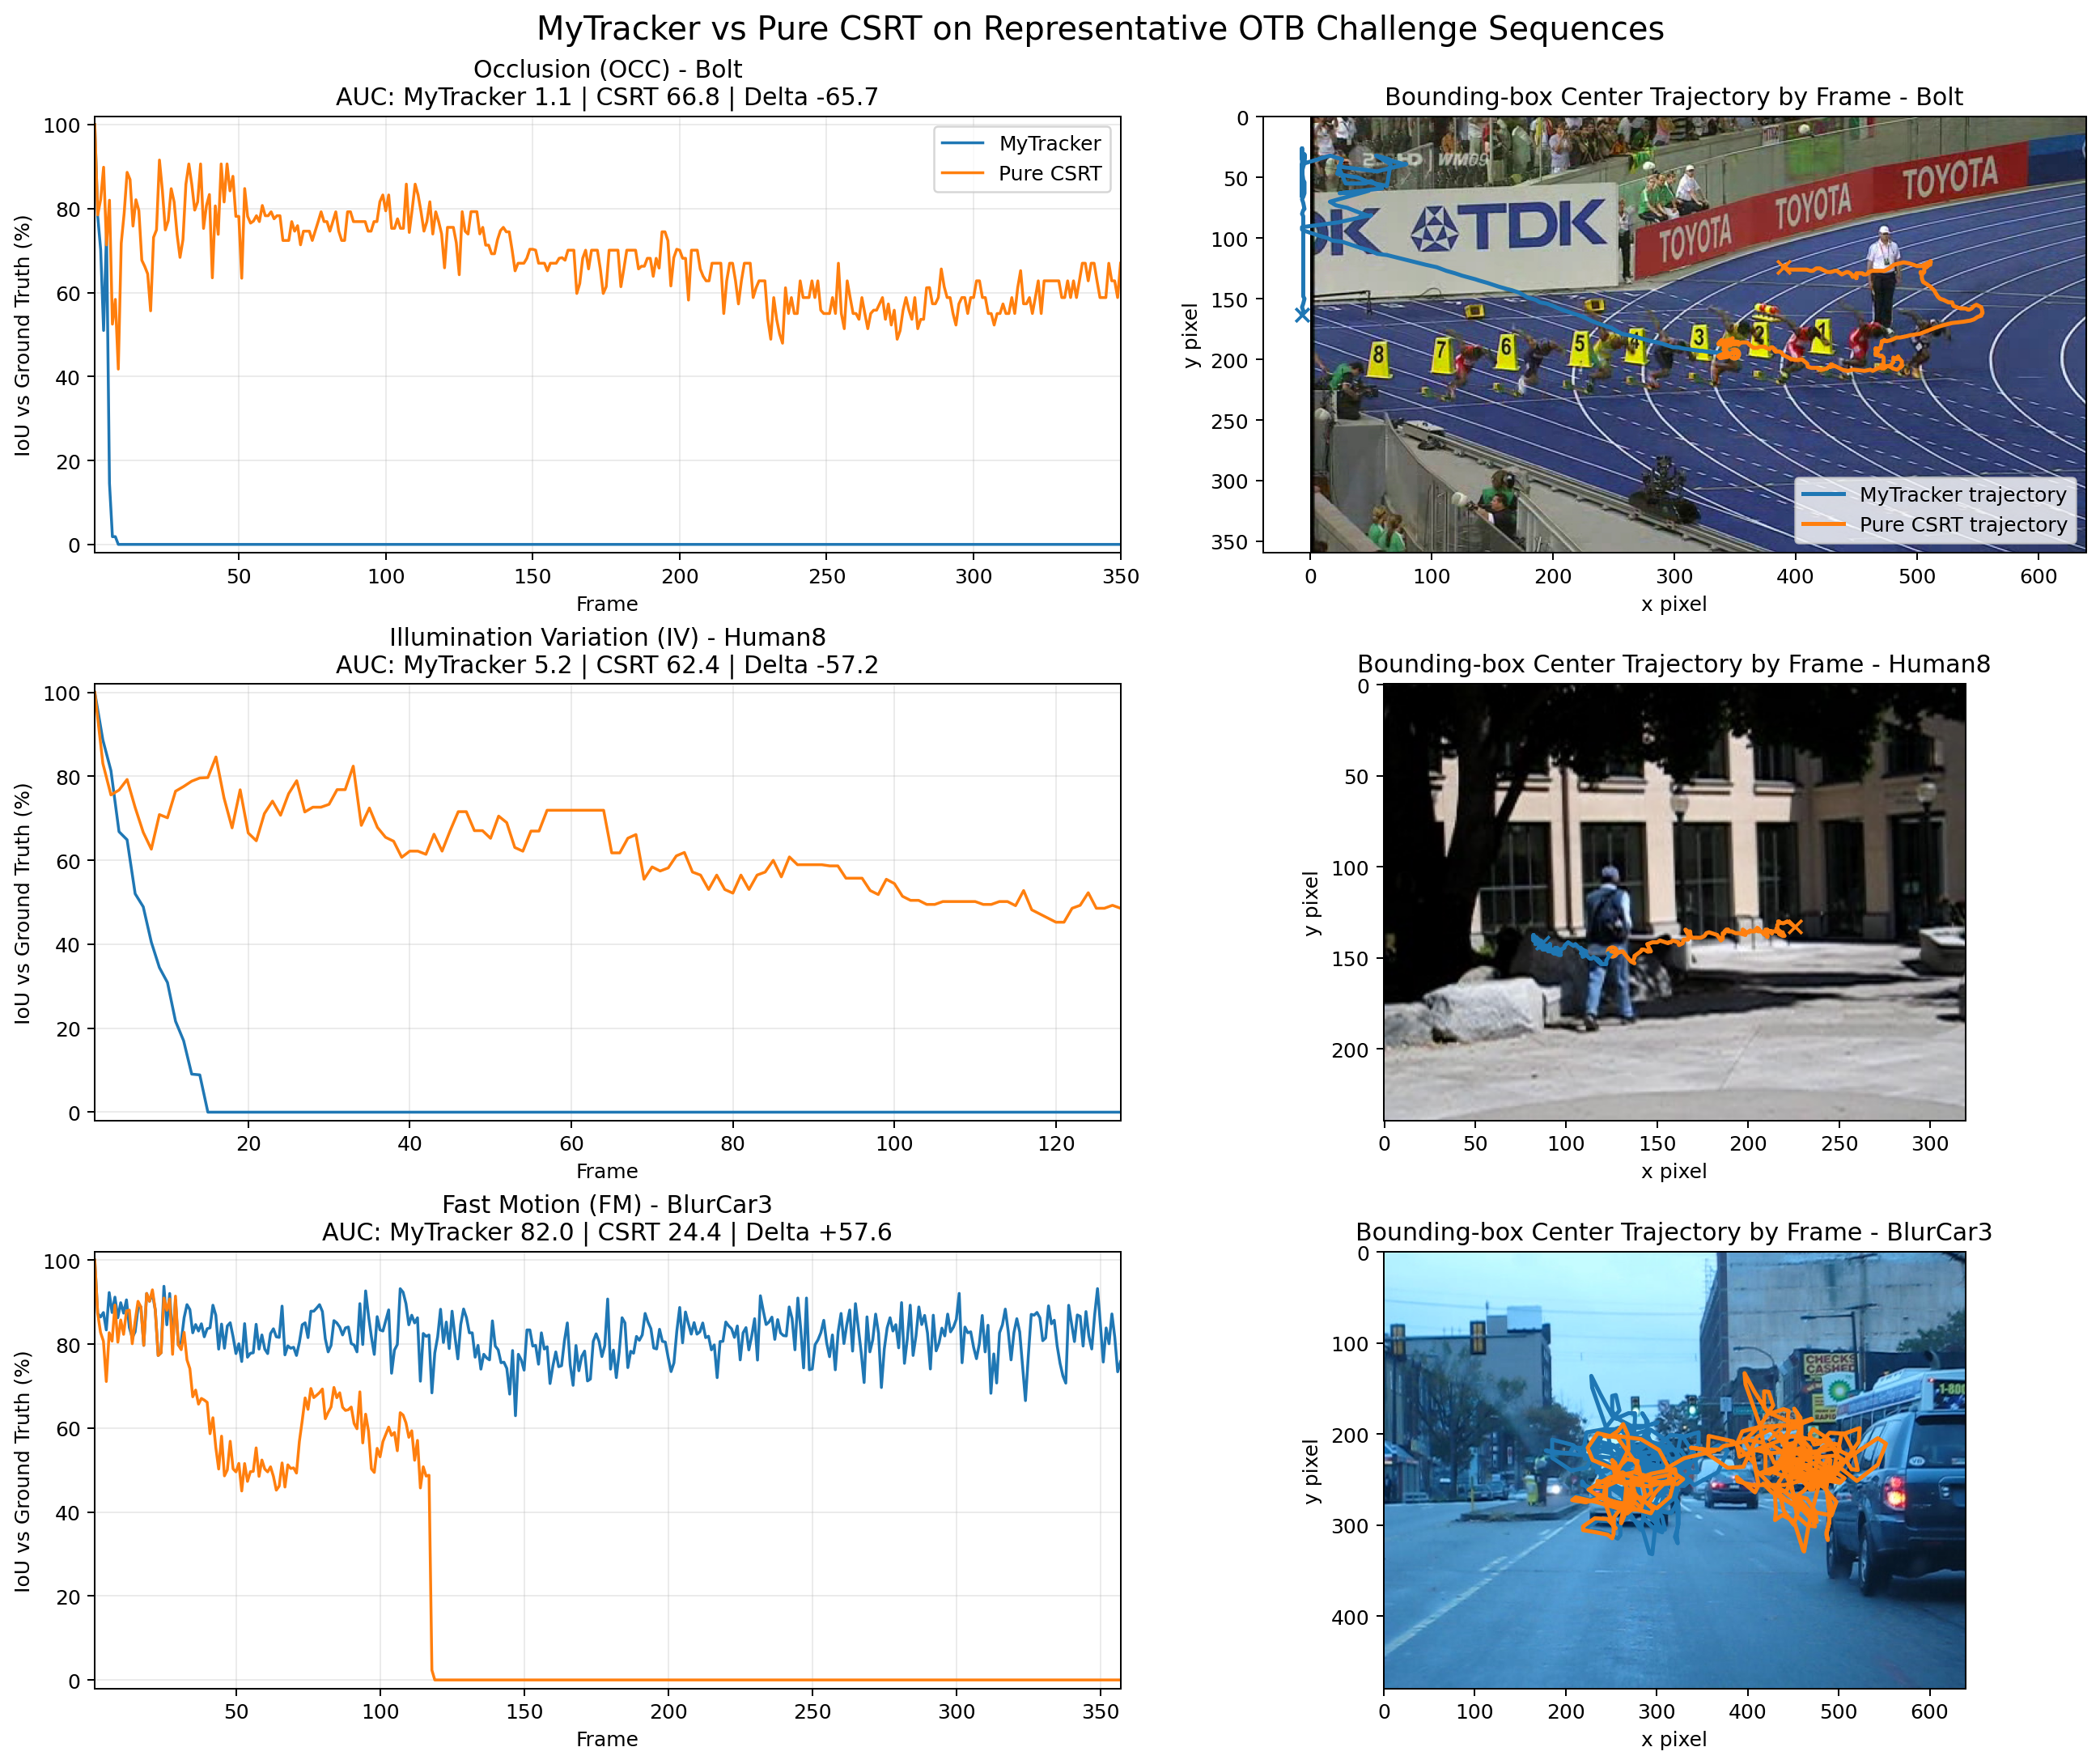
\includegraphics[width=0.94\columnwidth]{challenge_representative_mytracker_vs_csrt.png}
\captionof{figure}{Representative OTB100 challenge sequences comparing CA-CSRT and pure CSRT. The left panels show IoU over time, while the right panels show bounding-box center trajectories.}
\label{fig:otb_representative_challenges}
\end{center}
\vspace{-0.20cm}

Figure~\ref{fig:otb_representative_challenges} provides a complementary view on representative OTB100 sequences. CA-CSRT strongly improves over pure CSRT on \textit{BlurCar3} under fast motion (+57.6 AUC), where the pure CSRT trajectory becomes unstable after a period of tracking. However, CA-CSRT fails early on \textit{Bolt} under occlusion (-65.7 AUC) and \textit{Human8} under illumination variation (-57.2 AUC), while pure CSRT remains closer to the target in these cases. This mixed behavior is consistent with the modest average OTB100 gain in Table~\ref{tab:csrt_comparison_summary}: CA-CSRT improves average robustness, but it is not a universally dominant replacement for pure CSRT.

\subsection{Embedded Deployment Results on Jetson Nano}

To evaluate practical deployability, CA-CSRT is analyzed on Jetson Nano using accuracy-related and runtime-related summaries.

\noindent
\begin{minipage}{0.82\columnwidth}
\begin{minipage}[t]{0.48\linewidth}
\centering
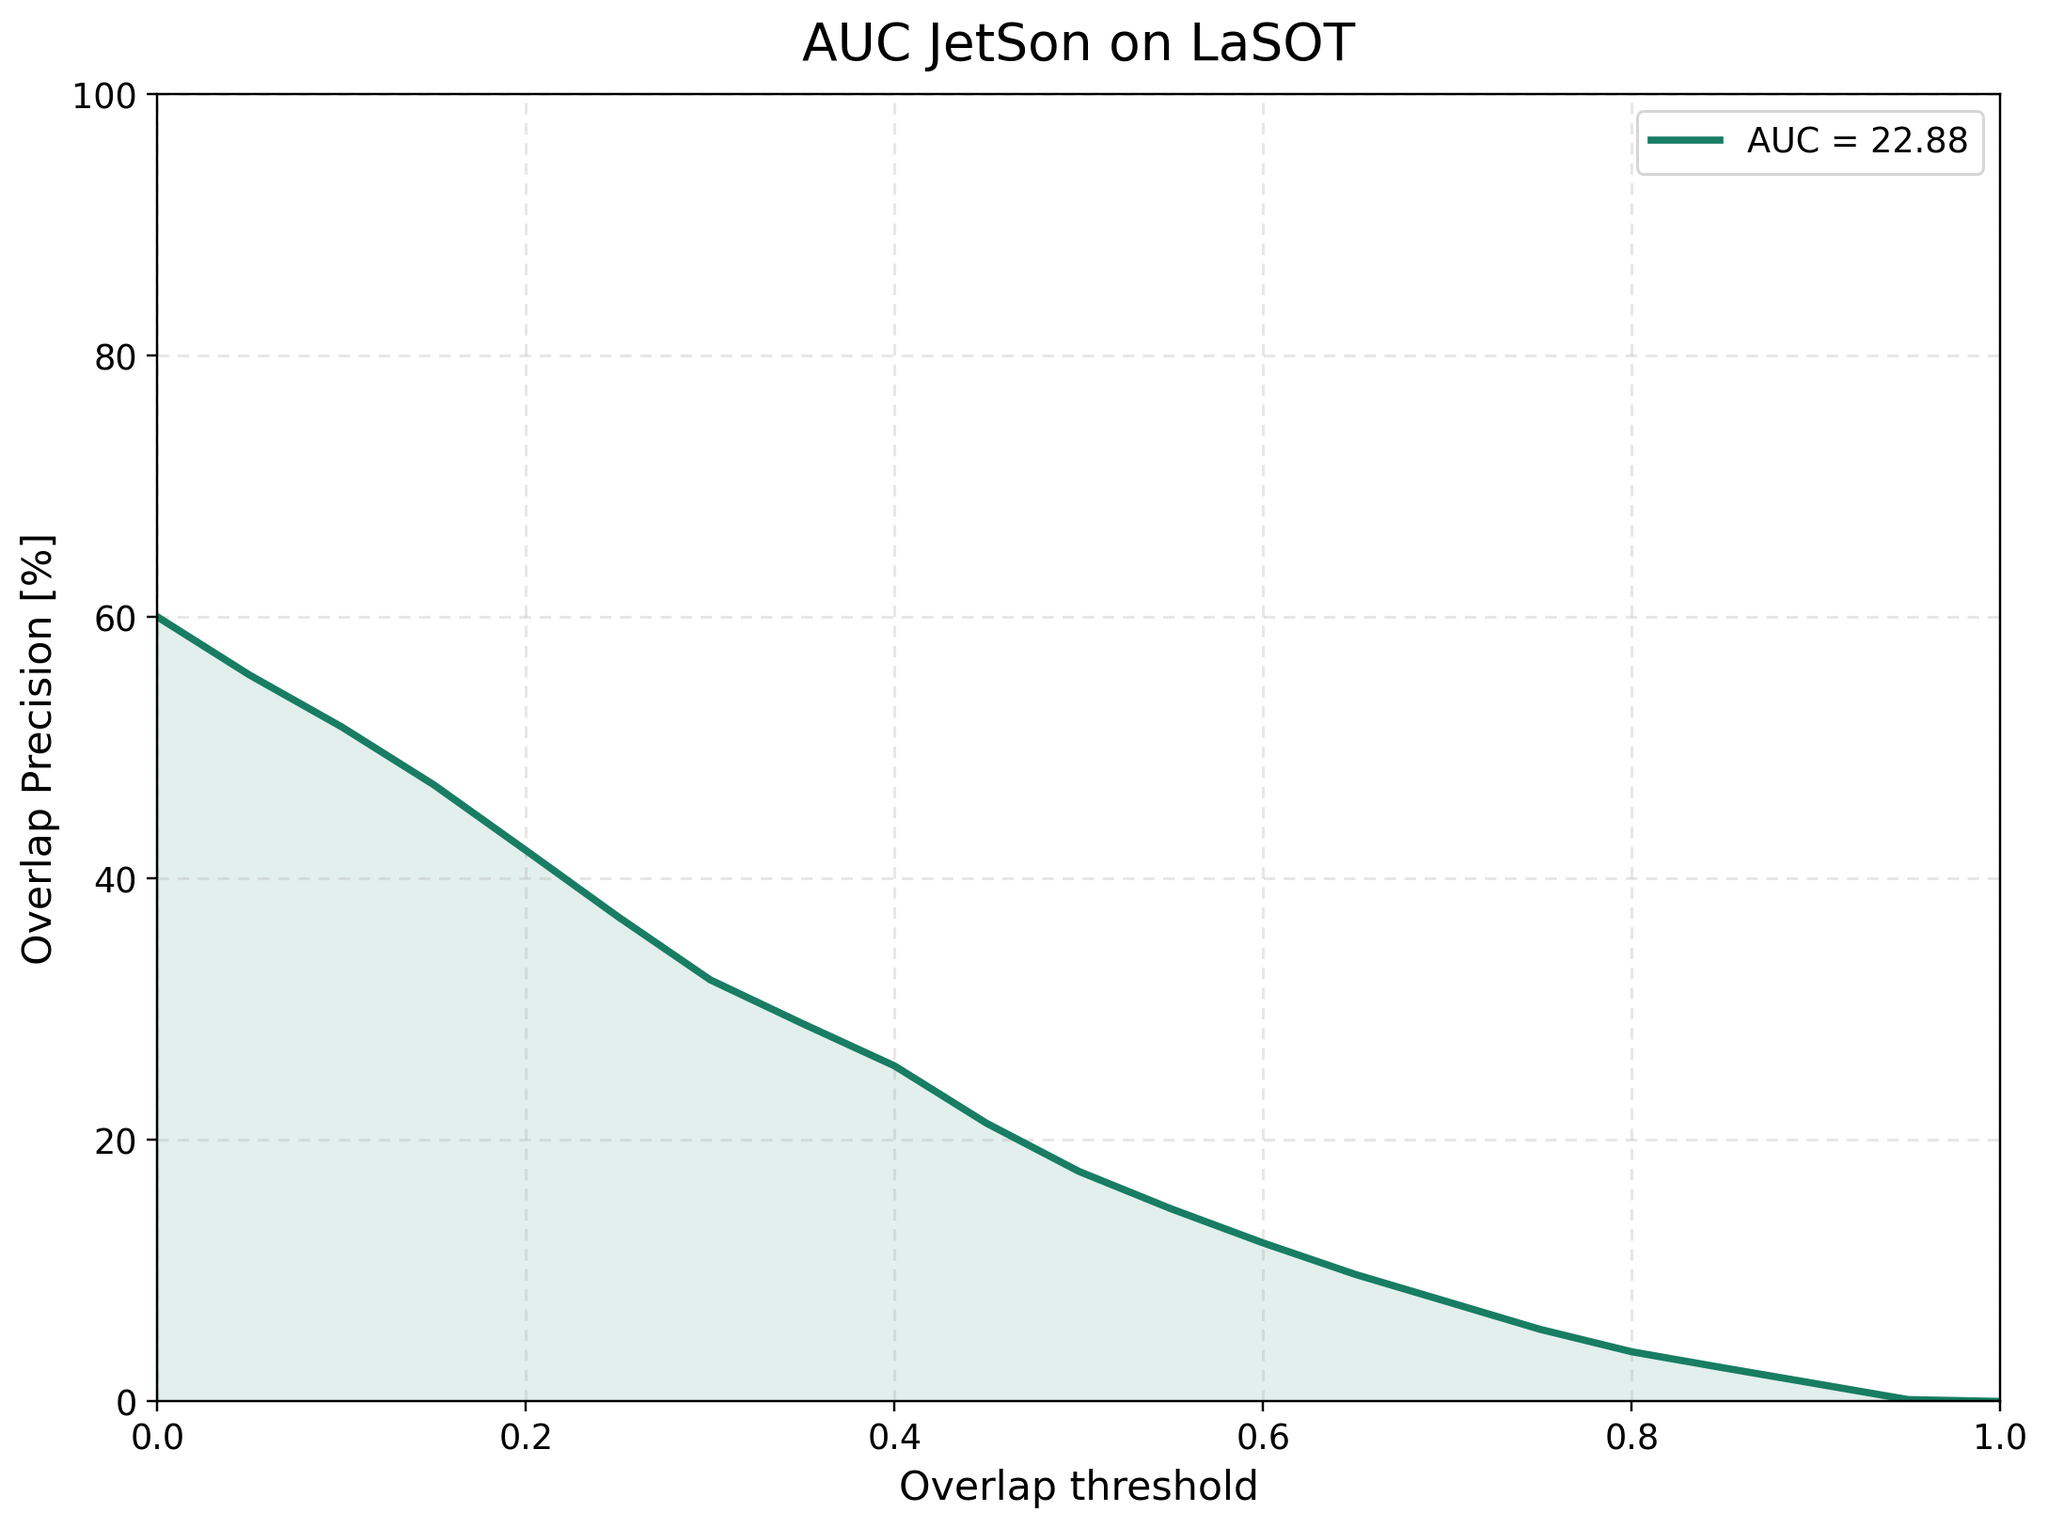
\includegraphics[width=\linewidth]{Jetson_Lasot_AUC.png}\\[-0.5em]
{\scriptsize (a) LaSOT AUC}
\end{minipage}
\hfill
\begin{minipage}[t]{0.48\linewidth}
\centering
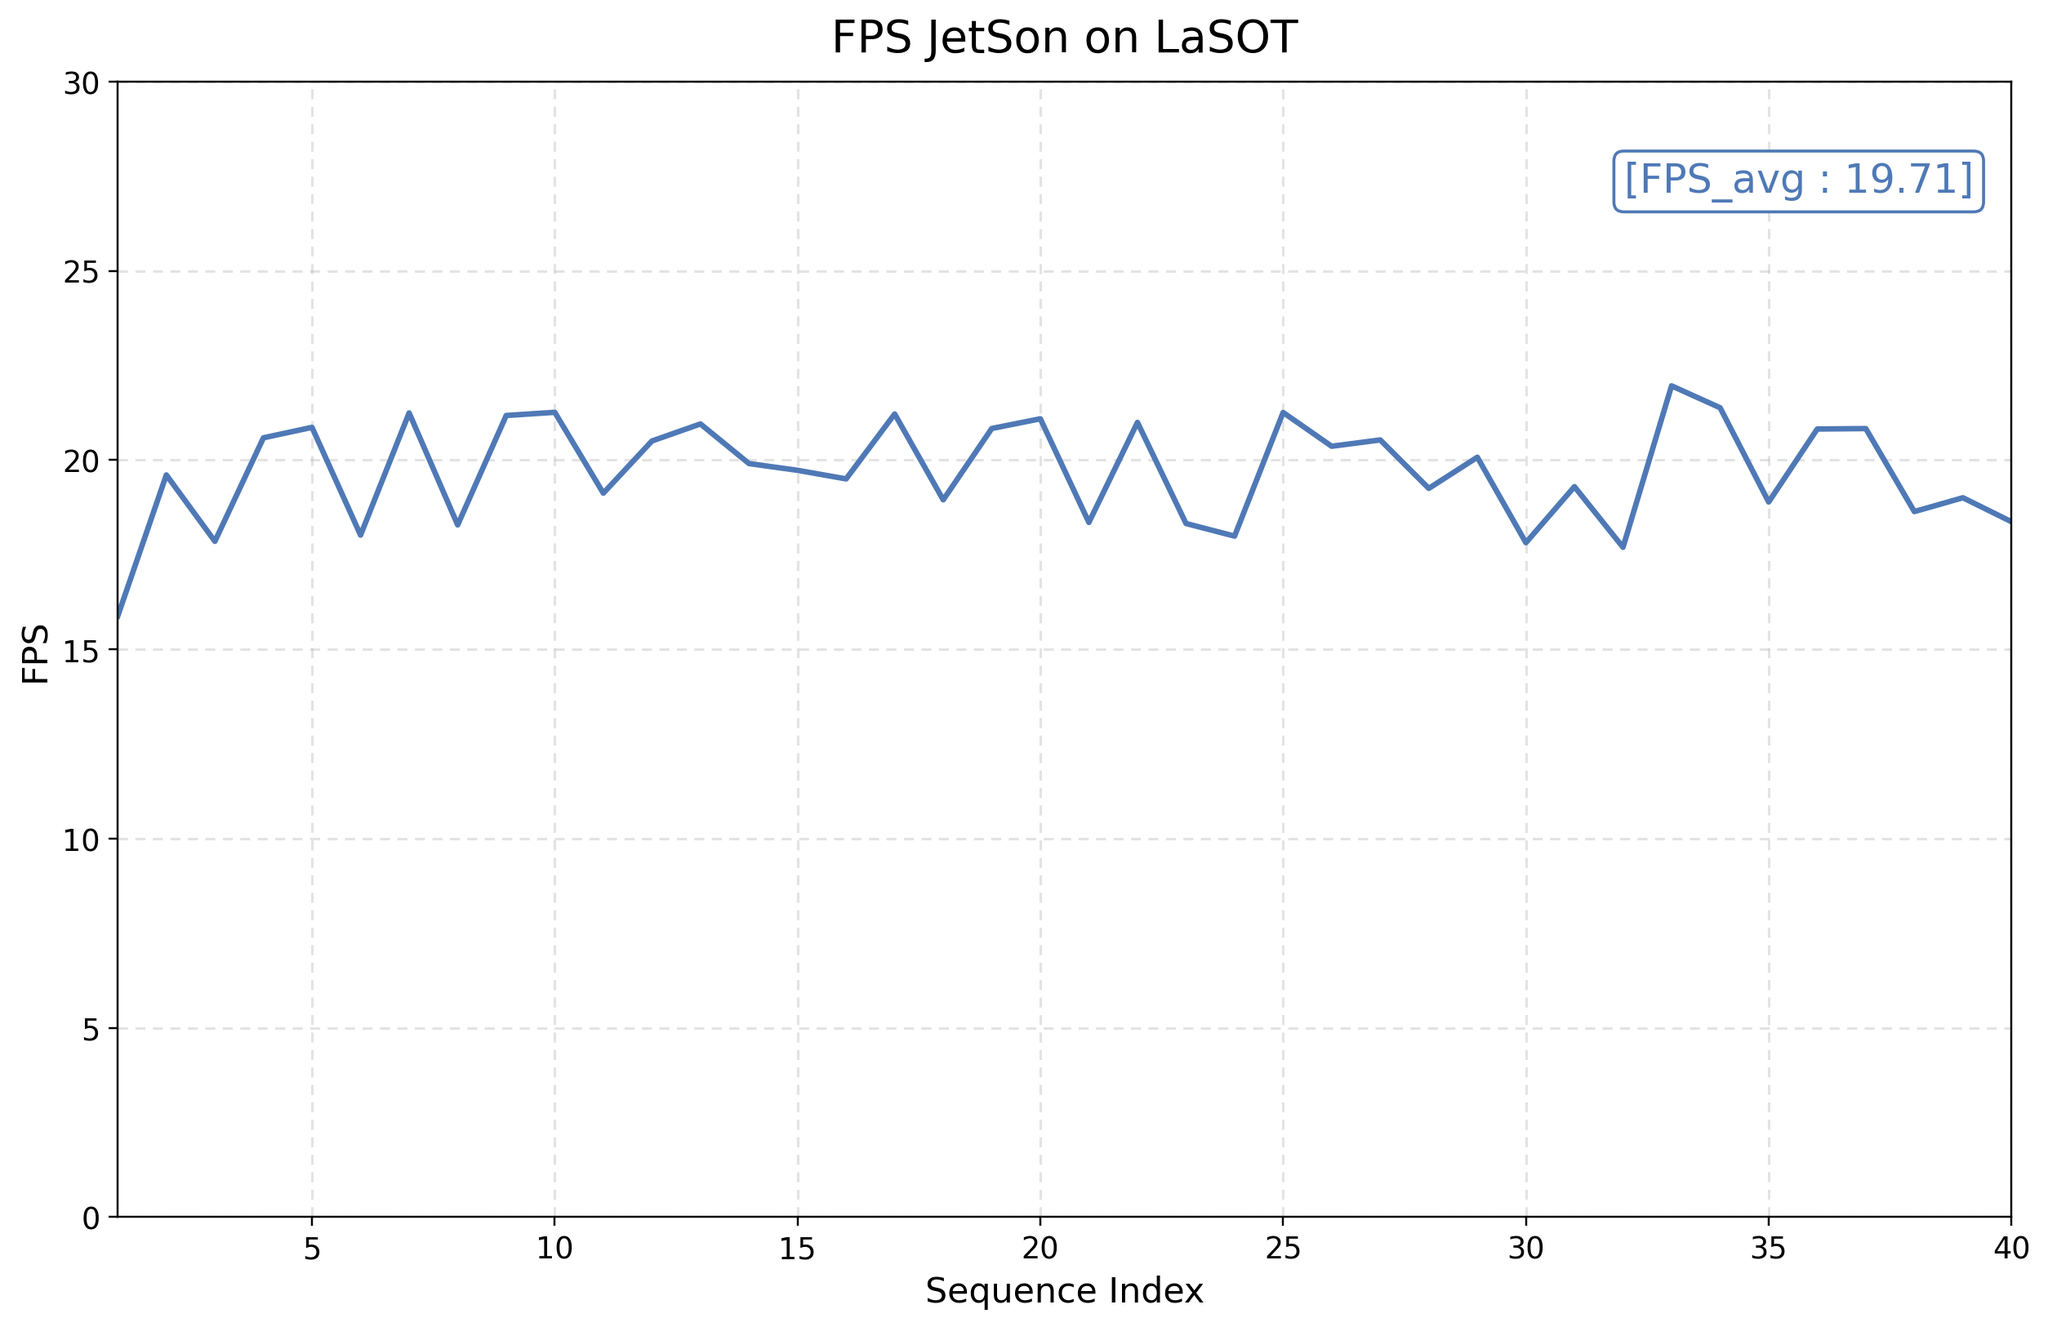
\includegraphics[width=\linewidth]{Jetson_Lasot_FPS.png}\\[-0.5em]
{\scriptsize (b) LaSOT FPS}
\end{minipage}

\vspace{0.1em}

\begin{minipage}[t]{0.48\linewidth}
\centering
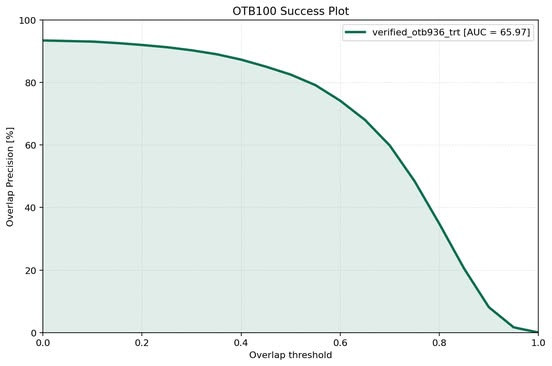
\includegraphics[width=\linewidth]{JetsonNano_OTB_SuccessPlot.png}\\[-0.5em]
{\scriptsize (c) OTB100 Success}
\end{minipage}
\hfill
\begin{minipage}[t]{0.48\linewidth}
\centering
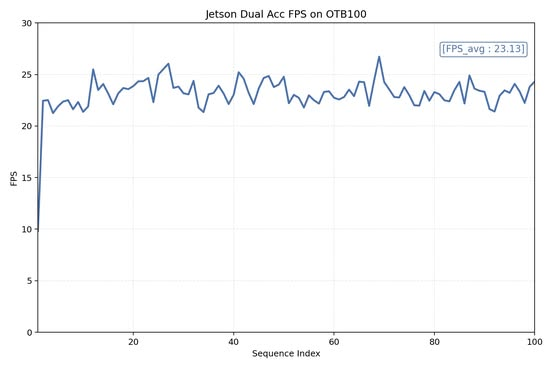
\includegraphics[width=\linewidth]{JetsonNano_OTB_FPS.png}\\[-0.5em]
{\scriptsize (d) OTB100 FPS}
\end{minipage}

\captionof{figure}{Compact Jetson Nano evaluation on LaSOT and OTB100.}
\label{fig:jetson_embedded_results}
\end{minipage}

The Jetson Nano results provide deployment-oriented evidence that CA-CSRT remains usable on resource-constrained hardware. FPS is interpreted as a practical deployment metric because runtime depends on implementation, hardware acceleration, preprocessing, and detector-assisted initialization or re-initialization. Therefore, the embedded results are used to support practical deployability rather than to rank CA-CSRT against all embedded trackers.

\subsection{Discussion}

Overall, the results support CA-CSRT as a robustness-efficiency enhancement rather than an absolutely dominant tracker. Compared with pure CSRT, it improves average AUC modestly on OTB100 and more clearly on the evaluated LaSOT subset. This trend supports the role of confidence-guided fusion and conservative update, especially when response ambiguity and accumulated model error become more influential.

The representative challenge-sequence analysis further supports this interpretation by showing that the proposed confidence-aware design is particularly meaningful in several difficult LaSOT cases, while also confirming that pure CSRT can remain competitive on some OTB100 sequences. The representative challenge analysis further clarifies this result: CA-CSRT is beneficial when motion prediction and confidence-controlled update prevent long drift, but it can still fail when an early incorrect estimate is reinforced and recovery is not achieved.

In the broader tracking and embedded-vision context, CA-CSRT keeps the efficient CSRT-family localization core and adds lightweight motion prediction, confidence estimation, and local scale refinement. The contribution is therefore a deployment-oriented improvement in robustness and efficiency, not a claim of absolute dominance over all trackers or all sequences.

\section{Conclusions}

This paper presented CA-CSRT, a confidence-aware enhancement of the CSRT-family tracking pipeline. The framework combines CSRT-based correlation localization, Kalman motion prediction, APCE-based response confidence, confidence-guided fusion, lightweight scale refinement, and confidence-controlled model update. Its central idea is to avoid treating every CSRT response peak as equally reliable: high-confidence responses can correct the motion prior and update the appearance model, while ambiguous responses are handled more conservatively.

Experiments show a modest average AUC improvement over pure CSRT on OTB100 and a larger improvement on the evaluated LaSOT subset. The FPS--AUC analysis and Jetson Nano evaluation further indicate practical runtime behavior for lightweight deployment, while also highlighting that speed should be interpreted with respect to hardware, implementation, and preprocessing choices.

These results should be interpreted as a robustness-efficiency improvement rather than absolute dominance, since pure CSRT remains competitive in several short-term cases. Future work will focus on more detailed attribute- and challenge-level analysis, tighter integration between motion prediction and appearance modeling, and further embedded optimization.

\section*{Acknowledgements}

The authors thank the open-source tracking community for providing datasets, benchmark protocols, tracker implementations, and software tools used in this work.

\begin{thebibliography}{99}

\bibitem{bolme2010}
D. S. Bolme, J. R. Beveridge, B. A. Draper, and Y. M. Lui,
``Visual object tracking using adaptive correlation filters,''
\textit{CVPR}, 2010.

\bibitem{henriques2015}
J. F. Henriques, R. Caseiro, P. Martins, and J. Batista,
``High-speed tracking with kernelized correlation filters,''
\textit{IEEE TPAMI}, 2015.

\bibitem{lukezic2017}
A. Lukežič et al.,
``Discriminative correlation filter with channel and spatial reliability,''
\textit{CVPR}, 2017.

\bibitem{danelljan2014}
M. Danelljan, G. Häger, F. Khan, and M. Felsberg,
``Accurate scale estimation for robust visual tracking,''
\textit{BMVC}, 2014.

\bibitem{kalman1960}
R. E. Kalman,
``A new approach to linear filtering and prediction problems,''
\textit{Journal of Basic Engineering}, 1960.

\bibitem{fan2019}
H. Fan, L. Lin, F. Yang, P. Chu, G. Deng, S. Yu, H. Bai, Y. Xu, C. Liao, and H. Ling,
``LaSOT: A high-quality benchmark for large-scale single object tracking,''
\textit{CVPR}, 2019.

\bibitem{wu2013}
Y. Wu, J. Lim, and M.-H. Yang,
``Online object tracking: A benchmark,''
\textit{CVPR}, 2013.

\bibitem{zhai2024}
J. Zhai, Z. Cheng, W. Zhang, D. Zhu, and W. Yang,
``Efficient object tracking on edge devices with MobileTrack,''
\textit{Journal of Visual Communication and Image Representation}, vol. 100, 104126, 2024.

\end{thebibliography}

\end{multicols}

\end{document}
